\chapter{Projektionen}\label{projektionen}
In diesem Kapitel betrachten wir die virtuelle Kamera in \emph{OpenGL}
und verschiedene Parallel- und Zentralprojektionen. Eine gute Quelle ist  \cite{angel:03}-
%
% Projektionen und Kameramodelle
%
\section{Projektionen und Kameramodelle}
Die Kamera in der Computergrafik k�nnen Sie sich als eine Lochkamera oder
\emph{Camera Obscura} vorstellen. Diese Metapher enth�lt die wesentlichen Eigenschaften,
die so gut wie alle Kameramodelle in der Computergrafik auszeichnen:
\begin{itemize}
\item die Position der Kamera ist gegeben durch die Koordinaten \emph{eines} Punkts in Weltkoordinaten;
\item der Bildausschnitt ist rechtwinklig;
\item der Sch�rfebereich der Kamera ist unendlich gro�.
\end{itemize}
Die den Kameramodellen zu Grunde liegende Mathematik wird \emph{Projektive Geometrie} oder
\emph{Darstellende Geometrie} genannt. Allerdings haben Sie in der Vorlesung nur einen
kurzen Einblick in diese F�cher bekommen.

Ganz entscheidend ist die Unterscheidung zwischen Welt- und Kamerakoordinatensystem. Bevor
eine Projektion, also eine Abbildung von drei- in einen zweidimensionalen Raum durchgef�hrt wird,
werden die Koordinaten unserer Objekte mit Hilfe einer Basistransformationsmatrix
in das Kamerakoordinatensystem umgerechnet. Die Kamera liegt im Ursprung dieses Koordinatensystems;
das macht viele Berechnungen in der Bildsynthese sp�ter viel einfacher.

Um zwischen den verschiedenen Koordinatensystemen zu unterscheiden, haben wir vereinbart, dass die
Achsen des Kamerakoordinatensystems mit $\vtr{u}$, $\vtr{v}$ und $\vtr{n}$ bezeichnet werden.

Nat�rlich ist es m�glich, diese drei Richtungen in Weltkoordinaten anzugeben. Aber mit Hilfe
des \emph{Projektionsvektors} $\vtr{p}$ und einem \emph{View-up-Vektor}\index{View-up-Vektor}
kann das Kamerakoordinatensystem berechnet werden:
\begin{enumerate}
\item $\vtr{n}$ ist gegeben durch $\vtr{n}=-\vtr{p}$;
\item $\vtr{u}$ ist orthogonal zur Ebene, die durch
$\vtr{n}$ und $\vtr{vup}$ gegeben ist:
\[
\vtr{u} = \frac{\vtr{vup} \times \vtr{n}}{\norm{\vtr{vup} \times \vtr{n}}};
\]
\item $\vtr{v}$ ist gegeben durch
\begin{equation}\label{nummFormel}
\vtr{v} = -\vtr{u} \times \vtr{n}=\vtr{n} \times \vtr{u}.
\end{equation}
\end{enumerate}
Die Formel \eqref{nummFormel} ist ein Beispiel f�r eine mathematische Formel mit einer Marke,
auf die wir mit \lstinline$eqref$ Bezug nehmen k�nnen.

Das Original des Utah Teapot befindet sich inzwischen
im Computer History Museum; in Abbildung \ref{mayakamera:teapot} auf
Seite \pageref{mayakamera:teapot} sehen Sie ein
Ausstellungsfoto als Beispiel f�r eine Abbildung mit Bezug dazu im Text.

\begin{figure}[ht]
\centering
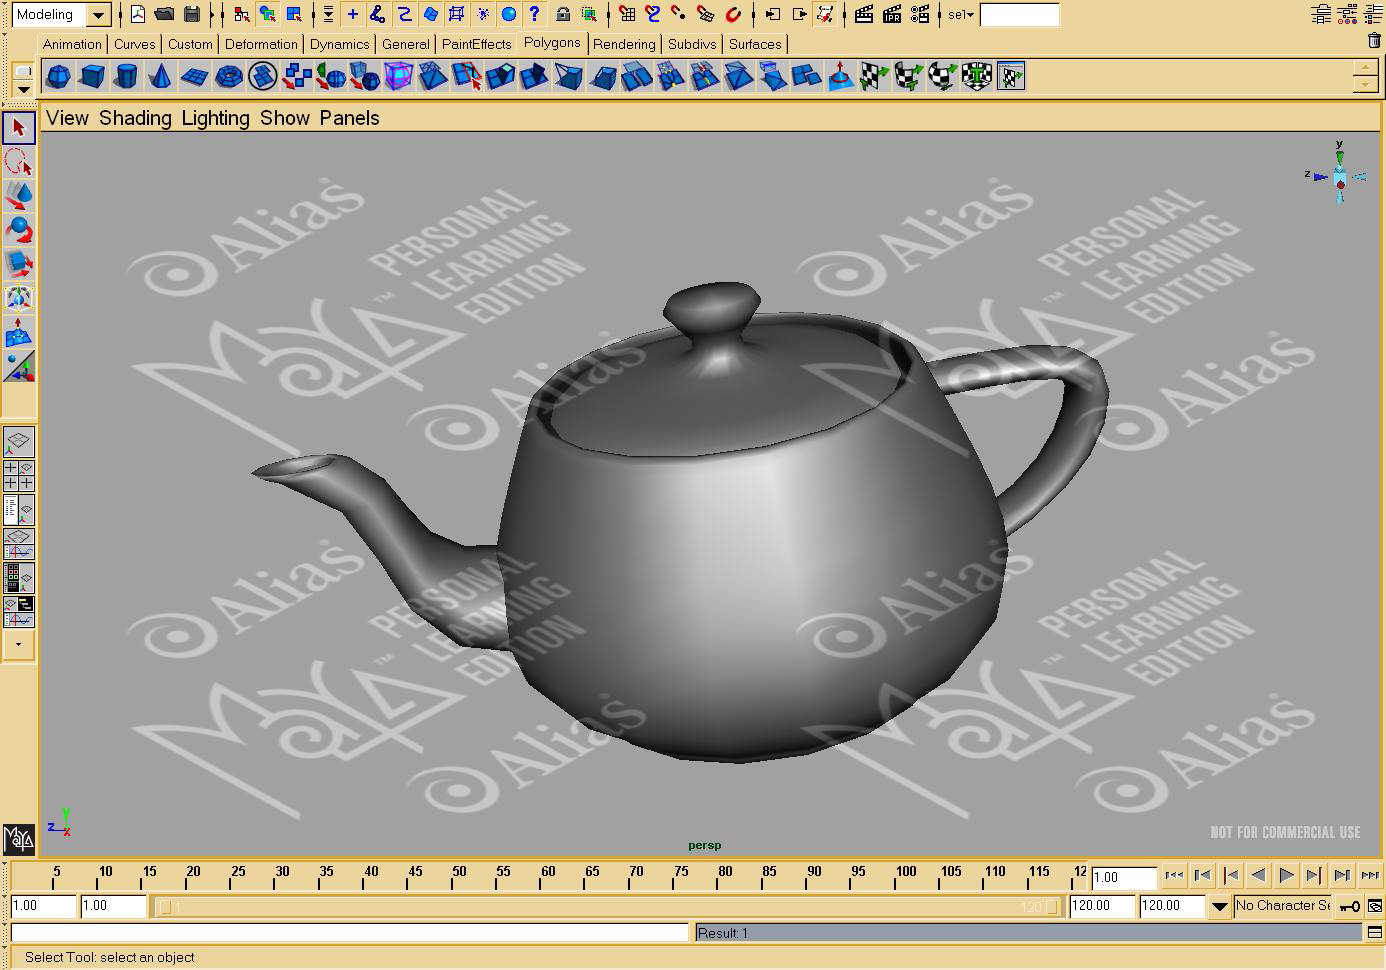
\includegraphics{mayateapot}
\caption{\label{mayakamera:teapot}Der \emph{Utah Teapot} in \emph{Maya}}
\end{figure}